\section{The Second Law of Thermodynamics}\label{sec:2nd_Law_Thermo}
\begin{definition}[\nth{2} Law of Thermodynamics]\label{def:2nd_Law_Thermo}
  The \emph{\nth{2} law of thermodynamics} states that the total \nameref{def:Entropy} of an \nameref{def:Isolated_System} can \textbf{never} decrease over time, and is constant if and only if all \nameref{def:Process}es are reversible.
  Isolated systems spontaneously evolve towards thermodynamic equilibrium, the state with maximum entropy.

  In terms of total \nameref{def:Energy} in a system, this law states that the total energy of the system is minimized at all times during a \nameref{def:Process}.

  \begin{remark}
    We do not discuss \nameref{def:Entropy} in this section.
    Rather, we discuss it in great detail in \Cref{sec:Entropy}.
  \end{remark}
\end{definition}

In more common terms, the \nameref{def:2nd_Law_Thermo} explains why some \nameref{def:Process}es only move in one direction.
For example, water going over a waterfall is \textit{technically} symmetric.
Meaning, that there is a chance the water will actually go back \textbf{up} the cliff.
However, the \nameref{def:2nd_Law_Thermo} explains that this reversal is so thermodynamically unfavorable that it will never happen.

Another example is a container of water that is greater than that of its surroundings.
For instance, the water is $\Temp = \SI{90}{\degreeF}$ and the surroundings are at $\Temp = \SI{20}{\degreeF}$.
The \nameref{def:2nd_Law_Thermo} explains why the heat always flows \textbf{out} of the water and to the surroundings, rather than the other way around.

This means that \textbf{energy is dispersed}.
This spread (dispersion) of energy is \nameref{def:Entropy}.

\begin{blackbox}
  \nameref{def:Energy} naturally flows from being concentrated in one place to another such that the dispersal of energy is maximized.
  This limits the \nameref{def:Work} that can be performed.
\end{blackbox}

\begin{definition}[Kelvin-Planck \nth{2} Law of Thermodynamics]\label{def:Kelvin_Planck-2nd_Law_Thermo}
  There are a variety of definitions of the \nth{2} law of thermodynamics.
  The one in \Cref{def:2nd_Law_Thermo} is just one of them.
  The \emph{Kelvin-Planck \nth{2} law of thermodynamics} states that it is impossible for any device that operates on a \nameref{def:Cycle} to receive heat form a single reservoir and use to to produce \nameref{def:Work}.

  \begin{remark}[Thermal Reservoir]\label{rmk:Thermal_Reservoir}
    A thermal source with a constant temperature.
    For example, the Earth, a large boiler, the air, a lake, or river are considered thermal reservoirs.
    More concretely, this means that if \nameref{def:Heat} is removed, there is no temperature change.
  \end{remark}
\end{definition}

\begin{definition}[Cycle]\label{def:Cycle}
  A \emph{cycle} is a \nameref{def:Process} whose ending state is the same as its starting state, allowing the process to continue again.

  \begin{remark}[Cyclic]\label{rmk:Cyclic}
    A \emph{cyclic} \nameref{def:Process} is one that behaves as a \nameref{def:Cycle}.
  \end{remark}
\end{definition}

\subsection{Thermodynamic Cycles}\label{subsec:Thermodynamic_Cycles}
Cycles absorb work, limiting the amount of energy that can be extracted.
You cannot perfectly convert \nameref{def:Heat} into \nameref{def:Work}.
This is because the cycle itself requires some amount of work to even occur.

\begin{example}[Textbook Problem 7.22]{Thermodynamic Cycles and Efficiency}
  Given a steam power plant, with a boiler, working shaft, condenser, and a source of water outputs $\Power = \SI{150}{\mega\watt}$ consumes coal at $\FlowRate{\Mass} = \SI{60}{\ton\per\hour}$.
  If the overall power available from coal is $\Power_{\text{Coal}} = \SI{30000}{\kilo\joule\per\kilo\gram}$, determine the overall efficiency of this plant?
  \tcblower{}
  The mass flowrate can be converted to kilograms, $\FlowRate{\Mass} = \SI{60000}{\kilo\gram\per\hour}$.

  \textbf{Concepts:} \\
  The efficiency can be defined as $\Efficiency = \frac{\FlowRate{\Work}_{\text{Net Out}}}{\FlowRate{\Heat}_{In}}$.

  \textbf{Explore:} \\
  There was no input work provided, so $\FlowRate{\Work}_{In} = 0$. \\

  \textbf{Solve:} \\
  So, we can find the heat in.
  \begin{align*}
    \FlowRate{\Heat}_{In} &= \FlowRate{\Mass} \Power_{\text{Coal}} \\
                          &= 1.8 \times 10^{9}\si{\kilo\joule\per\hour} \\
                          &= \SI{500}{\mega\watt}
  \end{align*}

  Now, to solve for the efficiency, $\Efficiency$.
  \begin{align*}
    \Efficiency &= \frac{\FlowRate{\Work}_{\text{Net Out}}}{\FlowRate{\Heat}_{In}} \\
                &= \frac{\SI{150}{\mega\watt}}{\SI{500}{\mega\watt}} \\
                &= 0.3
  \end{align*}

  \textbf{Validate:} \\
  Because $\Efficiency = 1 - \frac{\Heat_{Out}}{\Heat_{In}}$, we can say $\FlowRate{\Work}_{Net} = \FlowRate{\Heat}_{In} - \FlowRate{\Heat}_{Out}$.
  Plugging our known values in for $\FlowRate{\Heat}_{Out}$, we fine that $\FlowRate{\Heat}_{Out} = \SI{350}{\mega\watt}$.
  This is the same as the energy lost by the system, which means we are correct.

  \textbf{Generalize:} \\
  You must waste \nameref{def:Heat} in order to have a \nameref{def:Cycle}.
\end{example}

\subsection{Heat Engines}\label{subsec:Heat_Engines}
One common system we will see is the \nameref{fig:Heat_Engine}.
\begin{figure}[h!tbp]
  \centering
  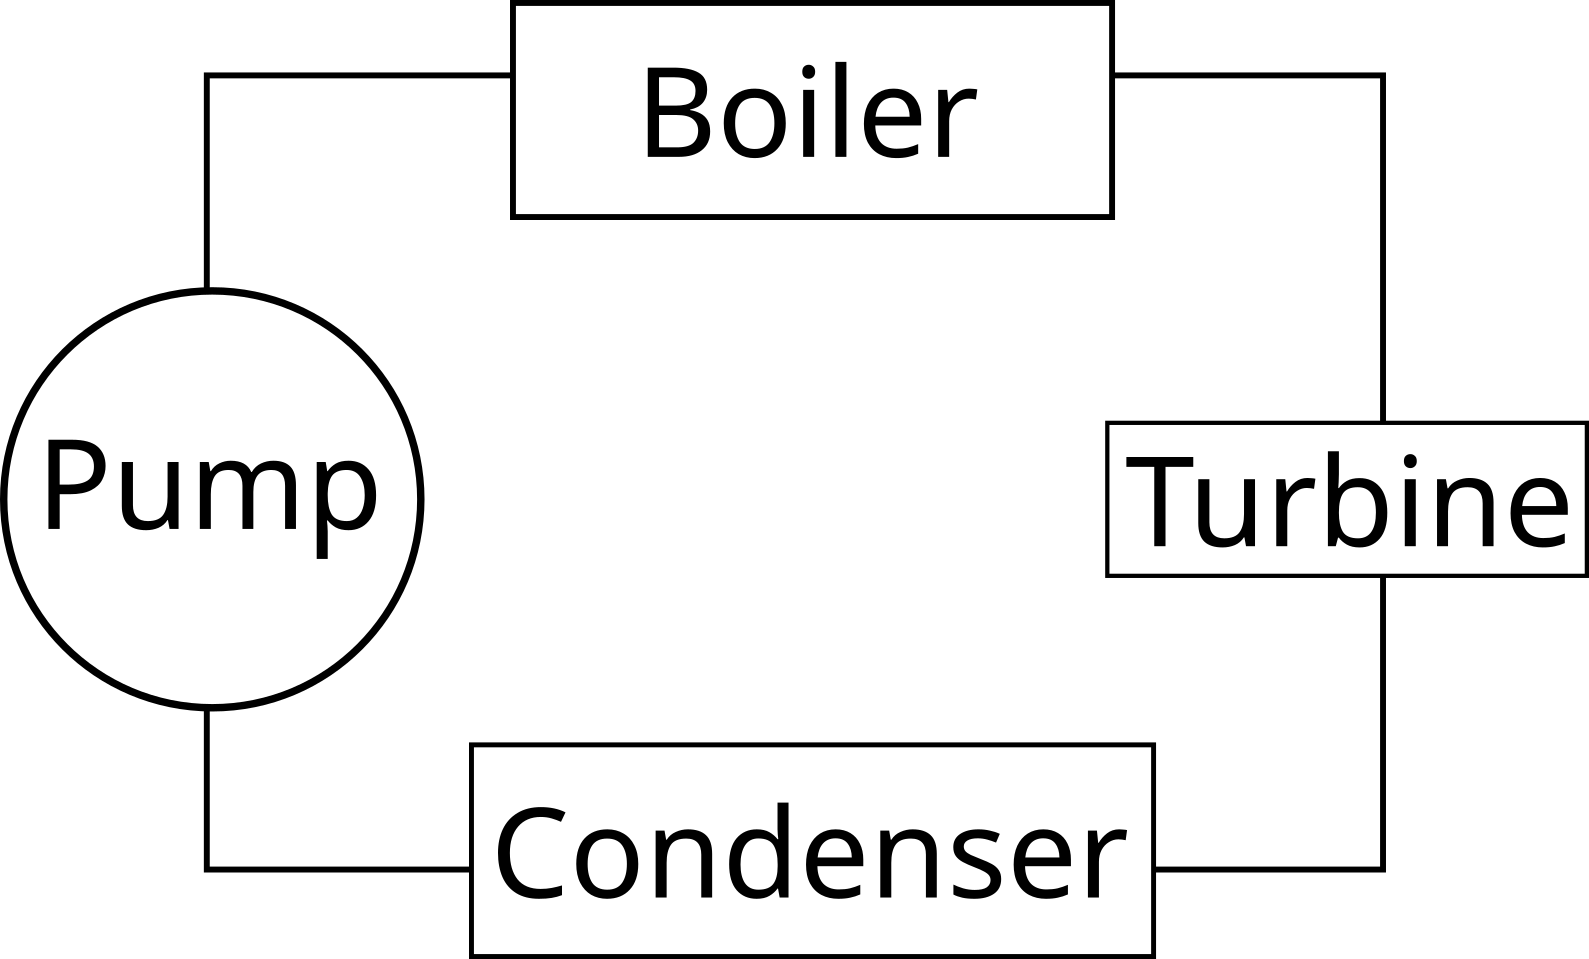
\includegraphics[scale=0.50]{./Heat_Engine_Schematic.png}
  % \input{./Drawings/MMAE_320-Thermo/Heat_Engine_Schematic.pdf_tex}
  \caption{Heat Engine}
  \label{fig:Heat_Engine}
\end{figure}

The boundary of the system is such that the entire system is contained.
This means that each element of the system is a different part of the thermodynamic energy balance.
\begin{itemize}[noitemsep]
\item The boiler takes the \nameref{def:Heat} in.
  Because this is typically the hot side of the \nameref{def:System}, we call this $\FlowRate{\Heat}_{H}$.
\item The turbine is for the \nameref{def:Work} out.
\item The condenser is for the \nameref{def:Heat} out.
  Because this is typically the cold side of the \nameref{def:System}, we call this $\FlowRate{\Heat}_{L}$.
\item The pump is for the \nameref{def:Work} in.
\end{itemize}

Thus, we can define the efficiency as shown in \Cref{eq:Energy_Efficiency-Heat_Engine}.
\begin{equation}\label{eq:Energy_Efficiency-Heat_Engine}
  \begin{aligned}
    \Efficiency &= \frac{\FlowRate{\Work}_{\text{Net Out}}}{\FlowRate{\Heat}_{H}} \\
    &= 1 - \frac{\FlowRate{\Heat}_{C}}{\FlowRate{\Heat}_{H}}
  \end{aligned}
\end{equation}

If we examine \Cref{eq:Energy_Efficiency-Heat_Engine}, we see that:
\begin{itemize}[noitemsep]
\item $\FlowRate{\Heat}_{H}$ sits on the boiler, which is at a higher temperature.
\item $\FlowRate{\Heat}_{C}$ sits on the condenser, which is at a lower temperature.
\end{itemize}
The greater the temperature difference between the system and its surroundings, the greater the efficiency of the \nameref{def:System}.

If there is no \nameref{def:Work} out, but work in is present, then \nameref{def:Energy} is being forced out of the lower temperature reservoir ($\FlowRate{\Heat}_{C}$) and put into the higher temperature reservoir.

%%% Local Variables:
%%% mode: latex
%%% TeX-master: "../MMAE_320-Thermo-Reference_Sheet"
%%% End:
